%versi 2 (8-10-2016)
\chapter{Pengujian Terhadap Kode Program Perangkat Lunak}
\label{lamp:B}

\section{Kode Program}
\label{kodeProgram:B}
\lstinputlisting[language=Java, caption=Extractor.java]{./Lampiran/Extractor.java}
\lstinputlisting[language=Java, caption=ClassExtractor.java]{./Lampiran/ClassExtractor.java}
\lstinputlisting[language=Java, caption=AttributeClassExtractor.java]{./Lampiran/AttributeClassExtractor.java}
\lstinputlisting[language=Java, caption=MethodClassExtractor.java]{./Lampiran/MethodClassExtractor.java}
\section{Hasil Latex}
\label{hasilLatex:B}
\lstinputlisting[language=TeX, caption=javadoctolatex.tex, label={javadoctolatex}]{./Lampiran/javadoctolatex.tex}
\section{Hasil PDF}
\label{hasilPDF:B}
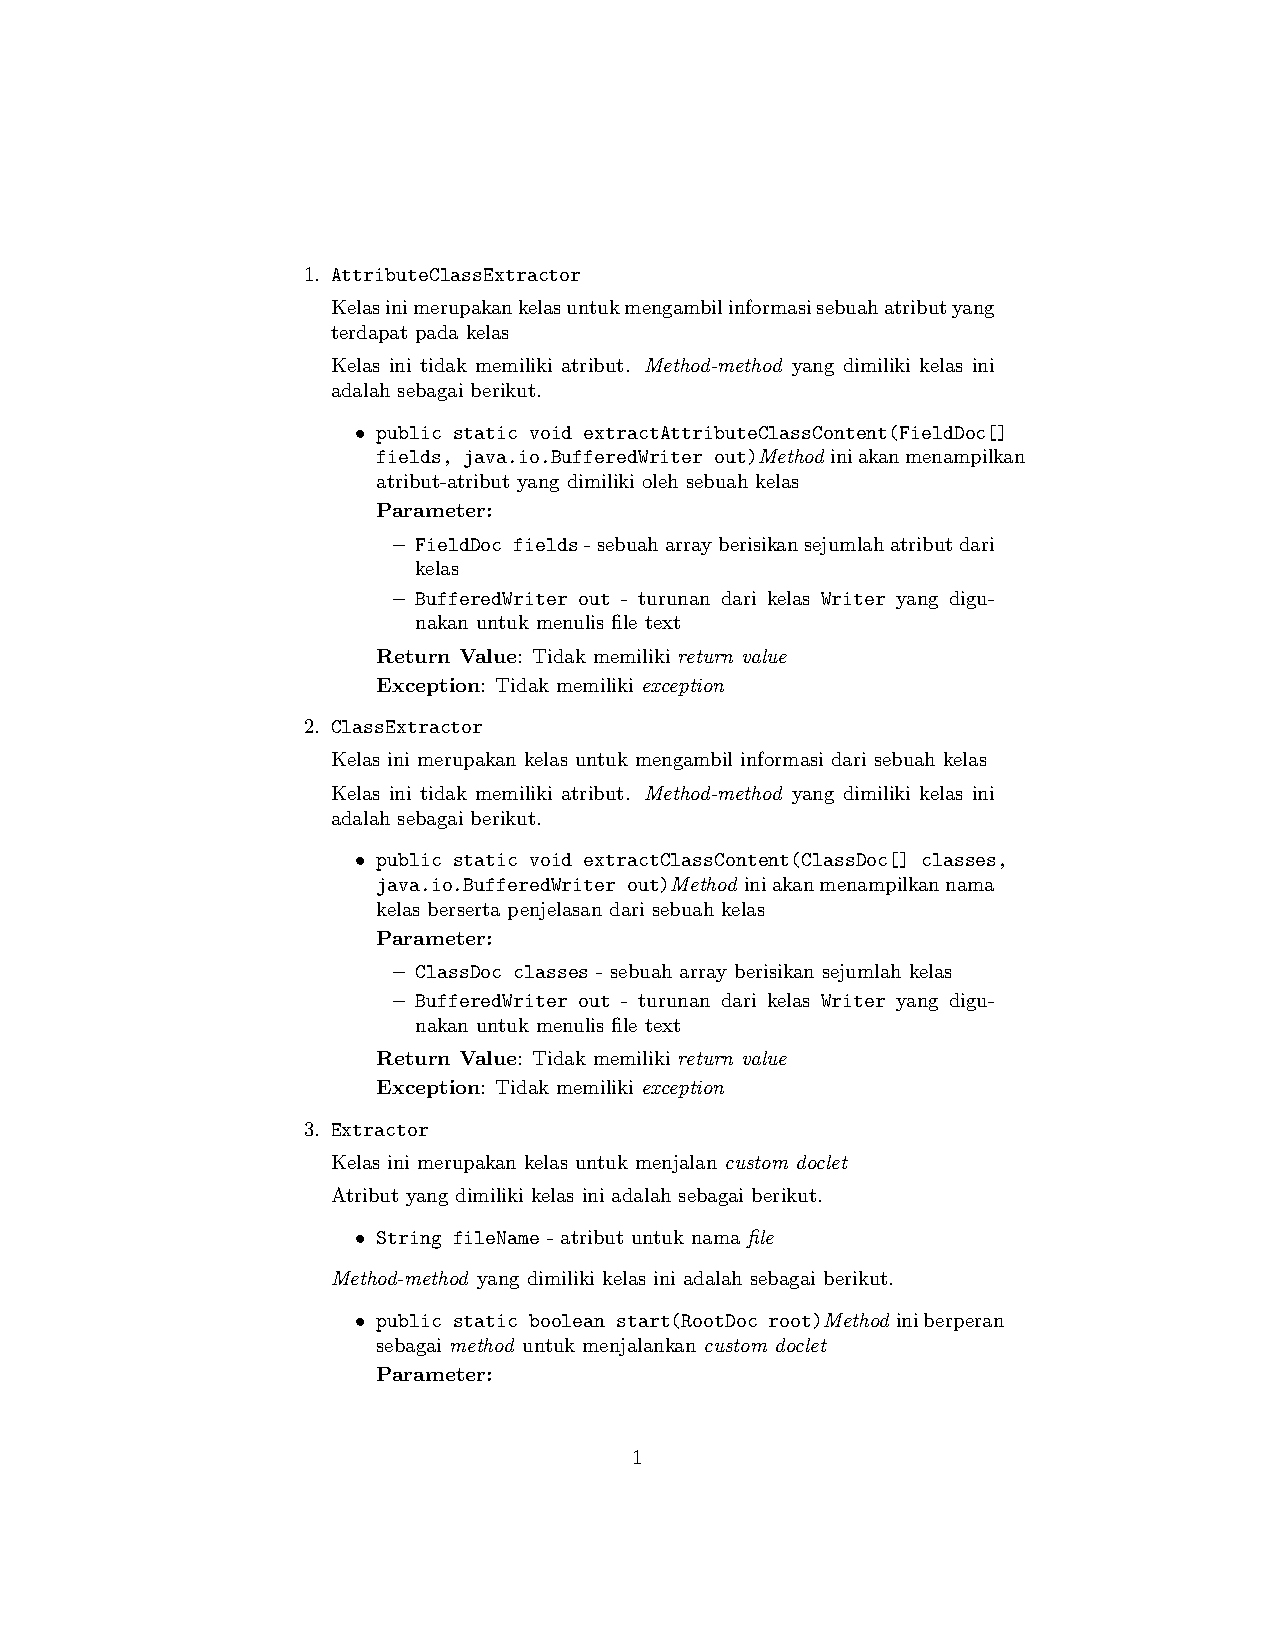
\includepdf[page=1-2]{./Lampiran/javadoctolatex.pdf}
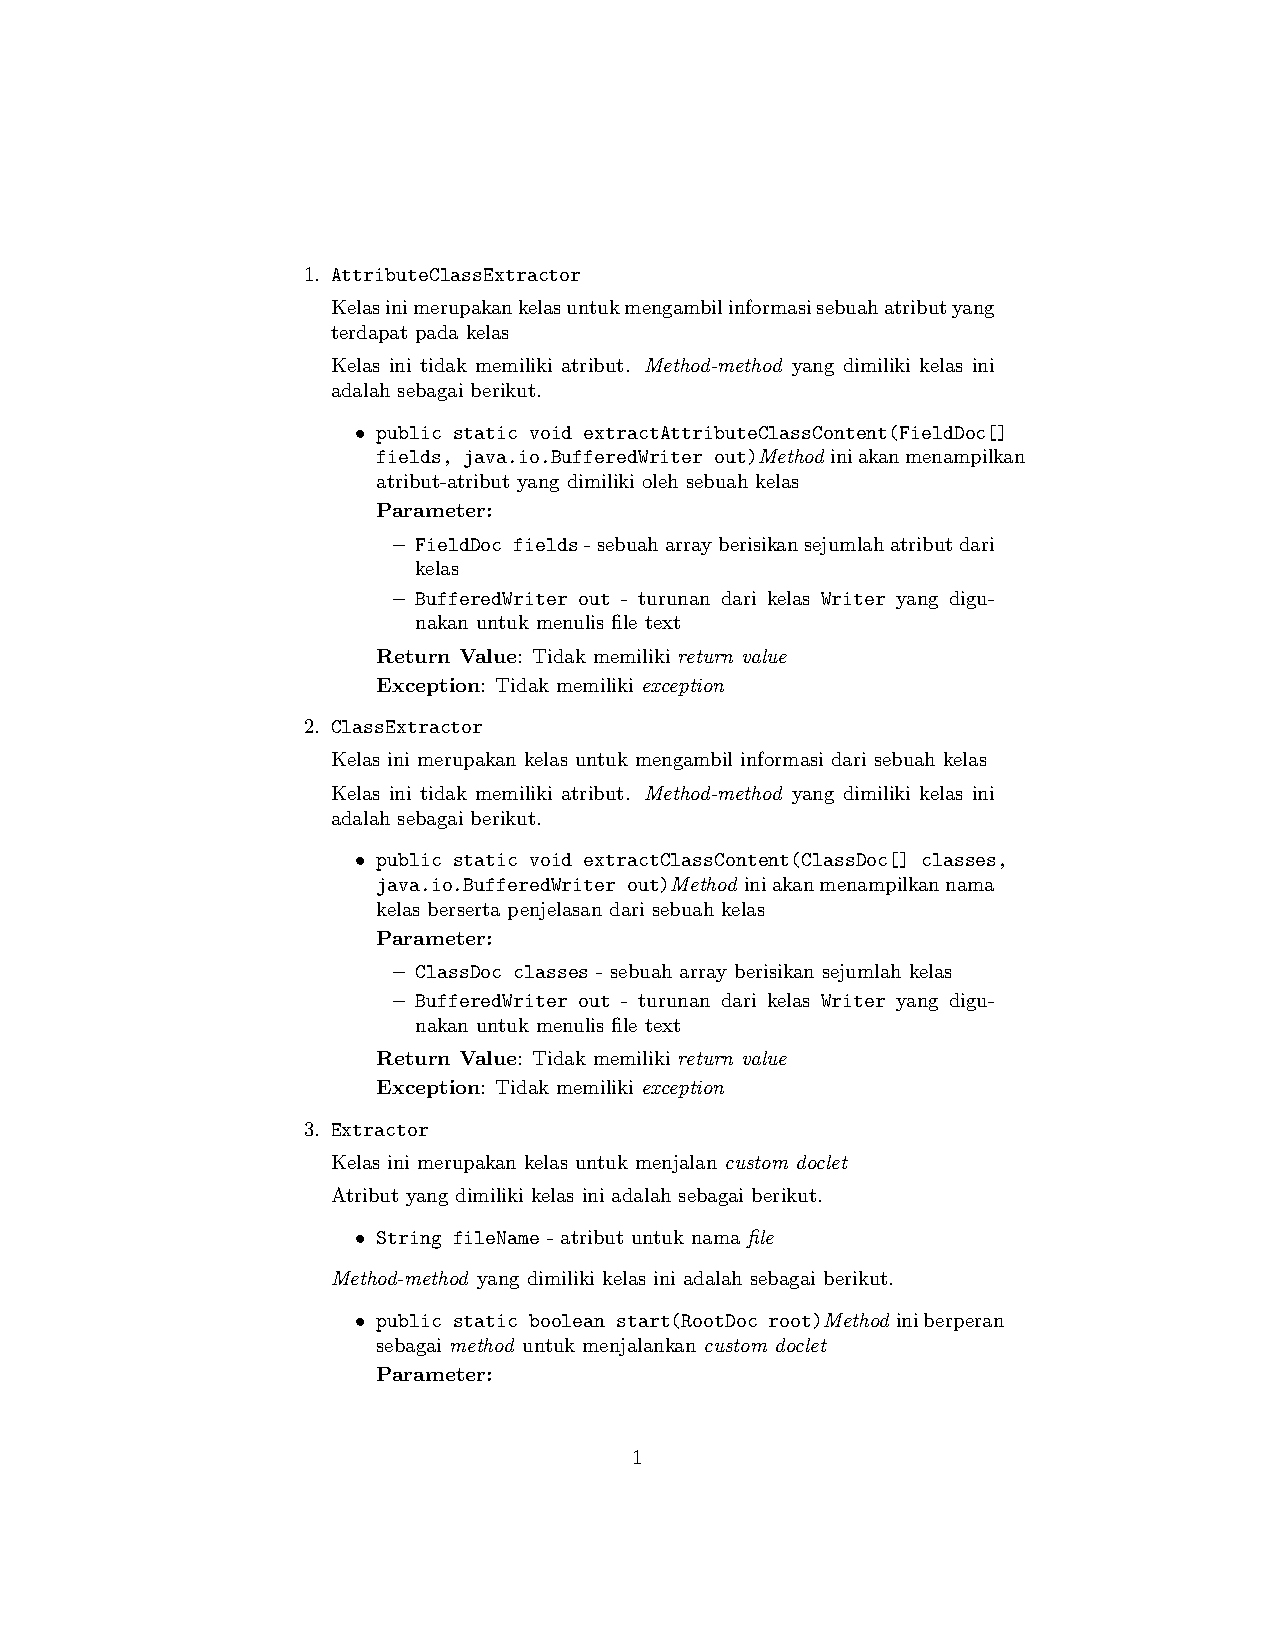
\includepdf[page=3,pagecommand={\null\vfill\captionof{figure}{javadoctolatex.pdf}}]{./Lampiran/javadoctolatex.pdf}

